\hfil
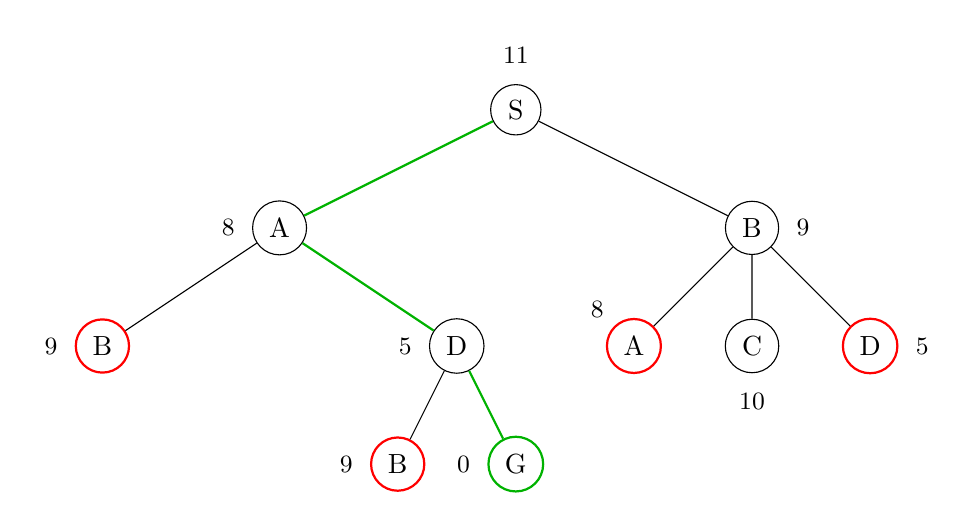
\begin{tikzpicture}[
    every node/.style = {shape=circle, draw=black, thin, align=center}
    ]
    \node[label={\small 11}] {S}
    child { node[label=left:{\small 8}] {A} edge from parent [draw=black!30!green, thick]   
        child { node[label=left:{\small 9}, draw=red, thick] {B} edge from parent [draw=black, thin] }
        child [missing]
        child [missing]
        child { node[label=left:{\small 5}] {D} edge from parent [draw=black!30!green, thick]
            child { node[label=left:{\small 9}, draw=red, thick] {B} edge from parent [draw=black, thin] }
            child { node[draw=black!30!green, thick, label=left:{\small 0}] {G} edge from parent [draw=black!30!green, thick] }
        }
    }
    child [missing]
    child [missing]
    child [missing]
    child { node[label=right:{\small 9}] {B} edge from parent [draw=black, thin] 
        child { node[label=above left:{\small 8}, draw=red, thick] {A} edge from parent [draw=black, thin] }
        child { node[label=below:{\small 10}] {C} edge from parent [draw=black, thin] }
        child { node[label=right:{\small 5}, draw=red, thick] {D} edge from parent [draw=black, thin] }
    };
\end{tikzpicture}

  